\section{Method}
\label{sec:videomamba}

\subsection{Preliminaries}

\noindent\textbf{SSM for 1D sequence.}
State Space Models (SSMs) are conceptualized based on continuous systems that map a 1D function or sequence, $x(t) \in \mathbb{R}^L \rightarrow y(t) \in \mathbb{R}^L $ through a hidden state  $h(t) \in \mathbb{R}^N$. Formally, SSMs employ the following ordinary differential equation (ODE) to model the input data:
\begin{align} 
h'(t) &= {\mathbf A}h(t) + {\mathbf B}x(t), \\
y(t) &= {\mathbf C}h(t), 
\end{align}
where ${\mathbf A} \in \mathbb{R}^{N\times N}$ represents the system's evolution matrix, and ${\mathbf B} \in \mathbb{R}^{N\times 1}, {\mathbf C} \in \mathbb{R}^{ N\times 1}$ are the projection matrices. This continuous ODE is approximated through discretization in modern SSMs. Mamba~\cite{gu2023mamba} is one of the discrete versions of the continuous system, which includes a timescale parameter ${\mathbf \Delta}$ to transform the continuous parameters ${\mathbf A}, {\mathbf B}$ to their discrete counterparts $\overline{{\mathbf A}}, \overline{{\mathbf B}}$. The transformation typically employs the zero-order hold (ZOH) method, defined by:
\begin{align} 
\overline{{\mathbf A}} &= \exp({\mathbf \Delta \mathbf A}), \\
\overline{{\mathbf B}} &= ({\mathbf \Delta \mathbf A})^{-1} (\exp({\mathbf \Delta \mathbf A}) - {\mathbf I}) \cdot {\mathbf \Delta \mathbf B} \\
h_t &= \overline{{\mathbf A}} h_{t-1} + \overline{{\mathbf B}} x_t, \\
y_t &= {\mathbf C}h_t.
\end{align}

Contrary to traditional models that primarily rely on linear time-invariant SSMs, Mamba distinguishes itself by implementing a Selective Scan Mechanism (S6) as its core SSM operator. Within S6, the parameters ${\mathbf B} \in \mathbb{R}^{B\times L \times N}$, ${\mathbf C} \in \mathbb{R}^{B\times L \times N}$, and ${\mathbf \Delta} \in \mathbb{R}^{B \times L \times D}$ are directly derived from the input data $x \in \mathbb{R}^{B \times L \times D}$, indicating an intrinsic capacity for contextual sensitivity and adaptive weight modulation.
Fig. \ref{fig:mamba_block}\red{a} shows the details of the Mamba block.

% \vspace{0.05cm}
\noindent\textbf{Bidirectional SSM for Vision.}
The original Mamba block, 
designed for 1D sequences, 
falls short for visual tasks requiring spatial awareness. 
Building on this, 
Vision Mamba introduces a bidirectional Mamba (B-Mamba) block in Fig. \ref{fig:mamba_block}\red{b},
which adapts bidirectional sequence modeling for vision-specific applications. 
This block processes flattened visual sequences through simultaneous forward and backward SSMs, enhancing its capacity for spatially-aware processing. 
In this work, 
we extend the B-Mamba block for 3D video understanding.


\begin{figure}[t]
    \centering
    \vspace{-0.3cm}
    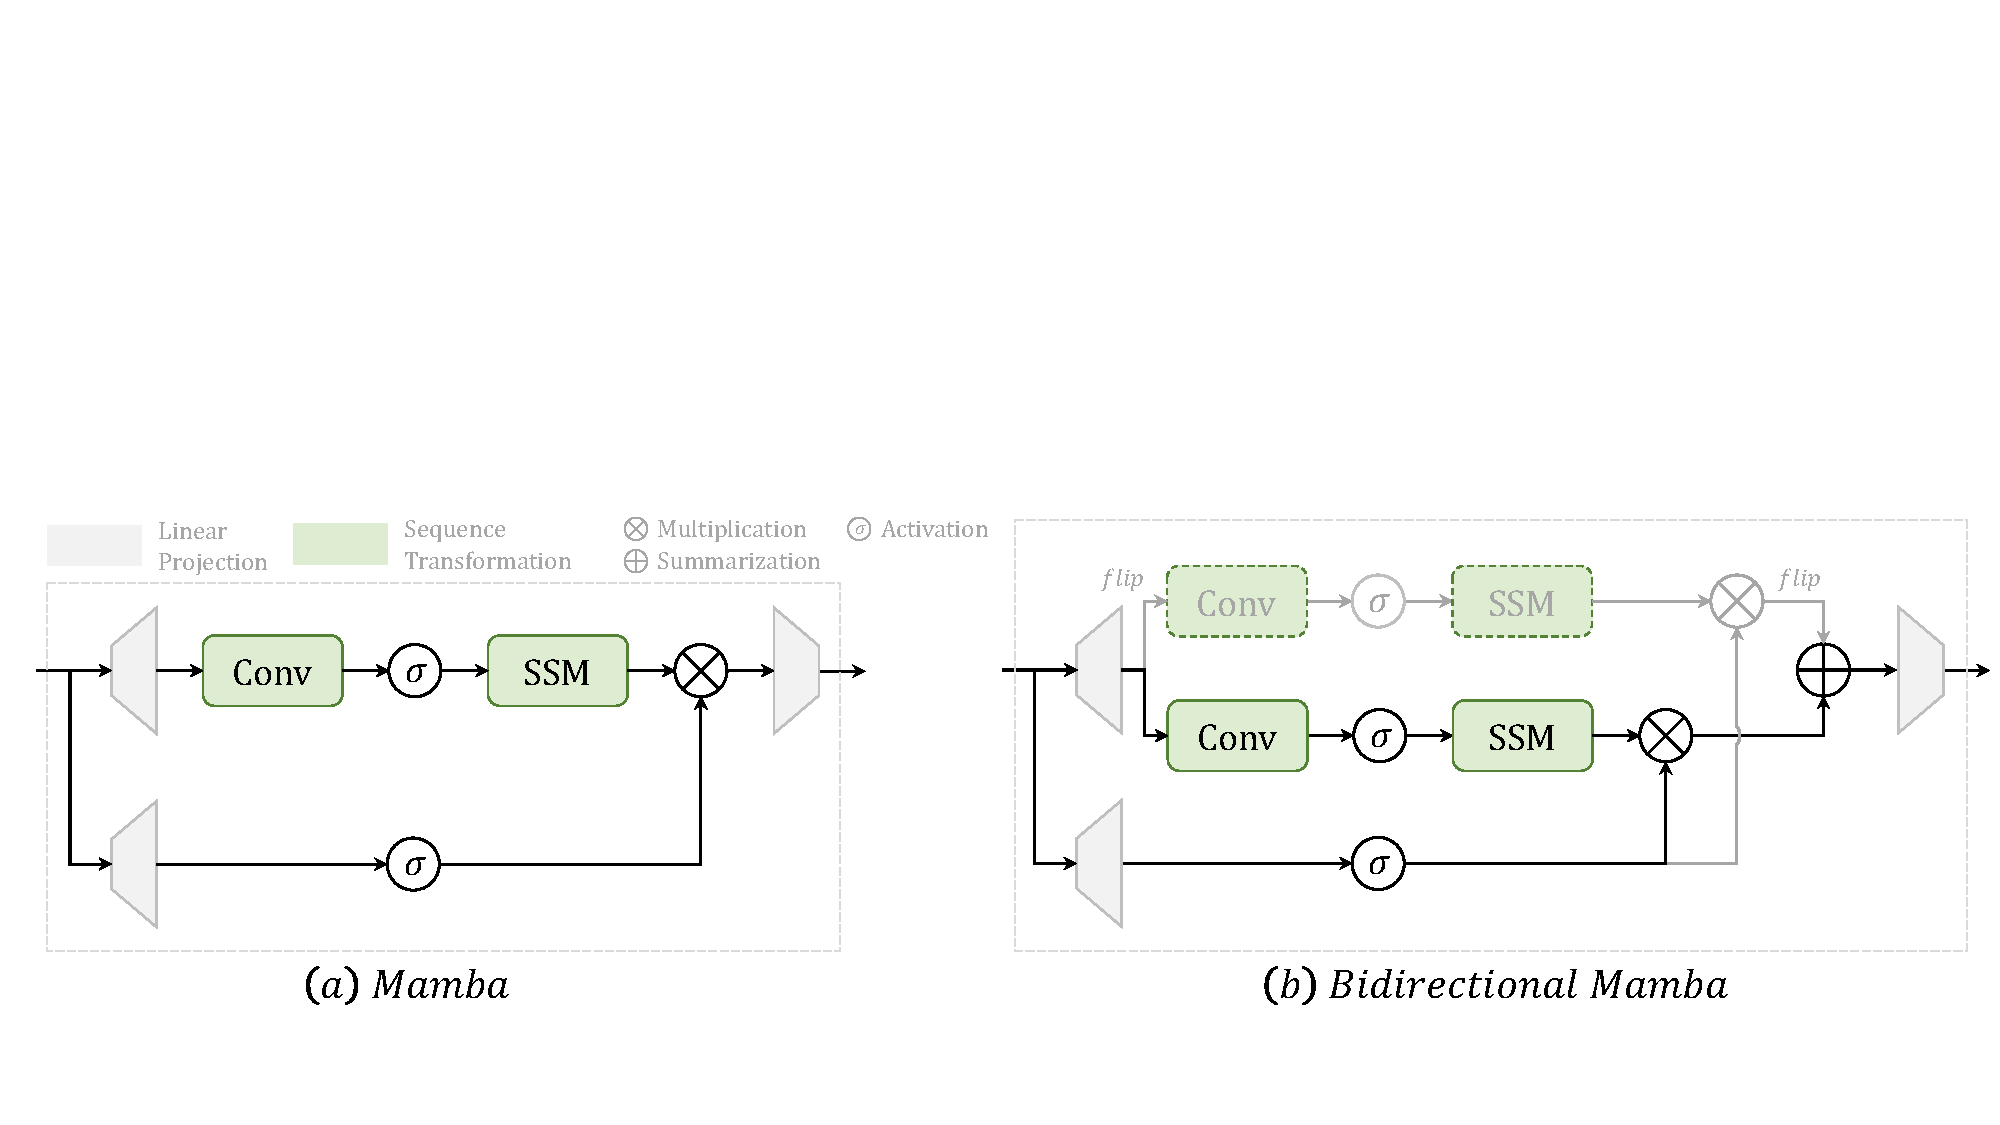
\includegraphics[width=1.0\textwidth]{figs/mamba_block.pdf}
    \vspace{-0.7cm}
    \caption{
    \textbf{Mamba blocks for 1D~\cite{gu2023mamba} and 2D~\cite{vim} sequence.} 
    We omit the initial normalization and the final residual for simplification.
    }
    \label{fig:mamba_block}
    \vspace{-0.3cm}
\end{figure}

\begin{figure}[t]
    \centering
    % \vspace{-0.3cm}
    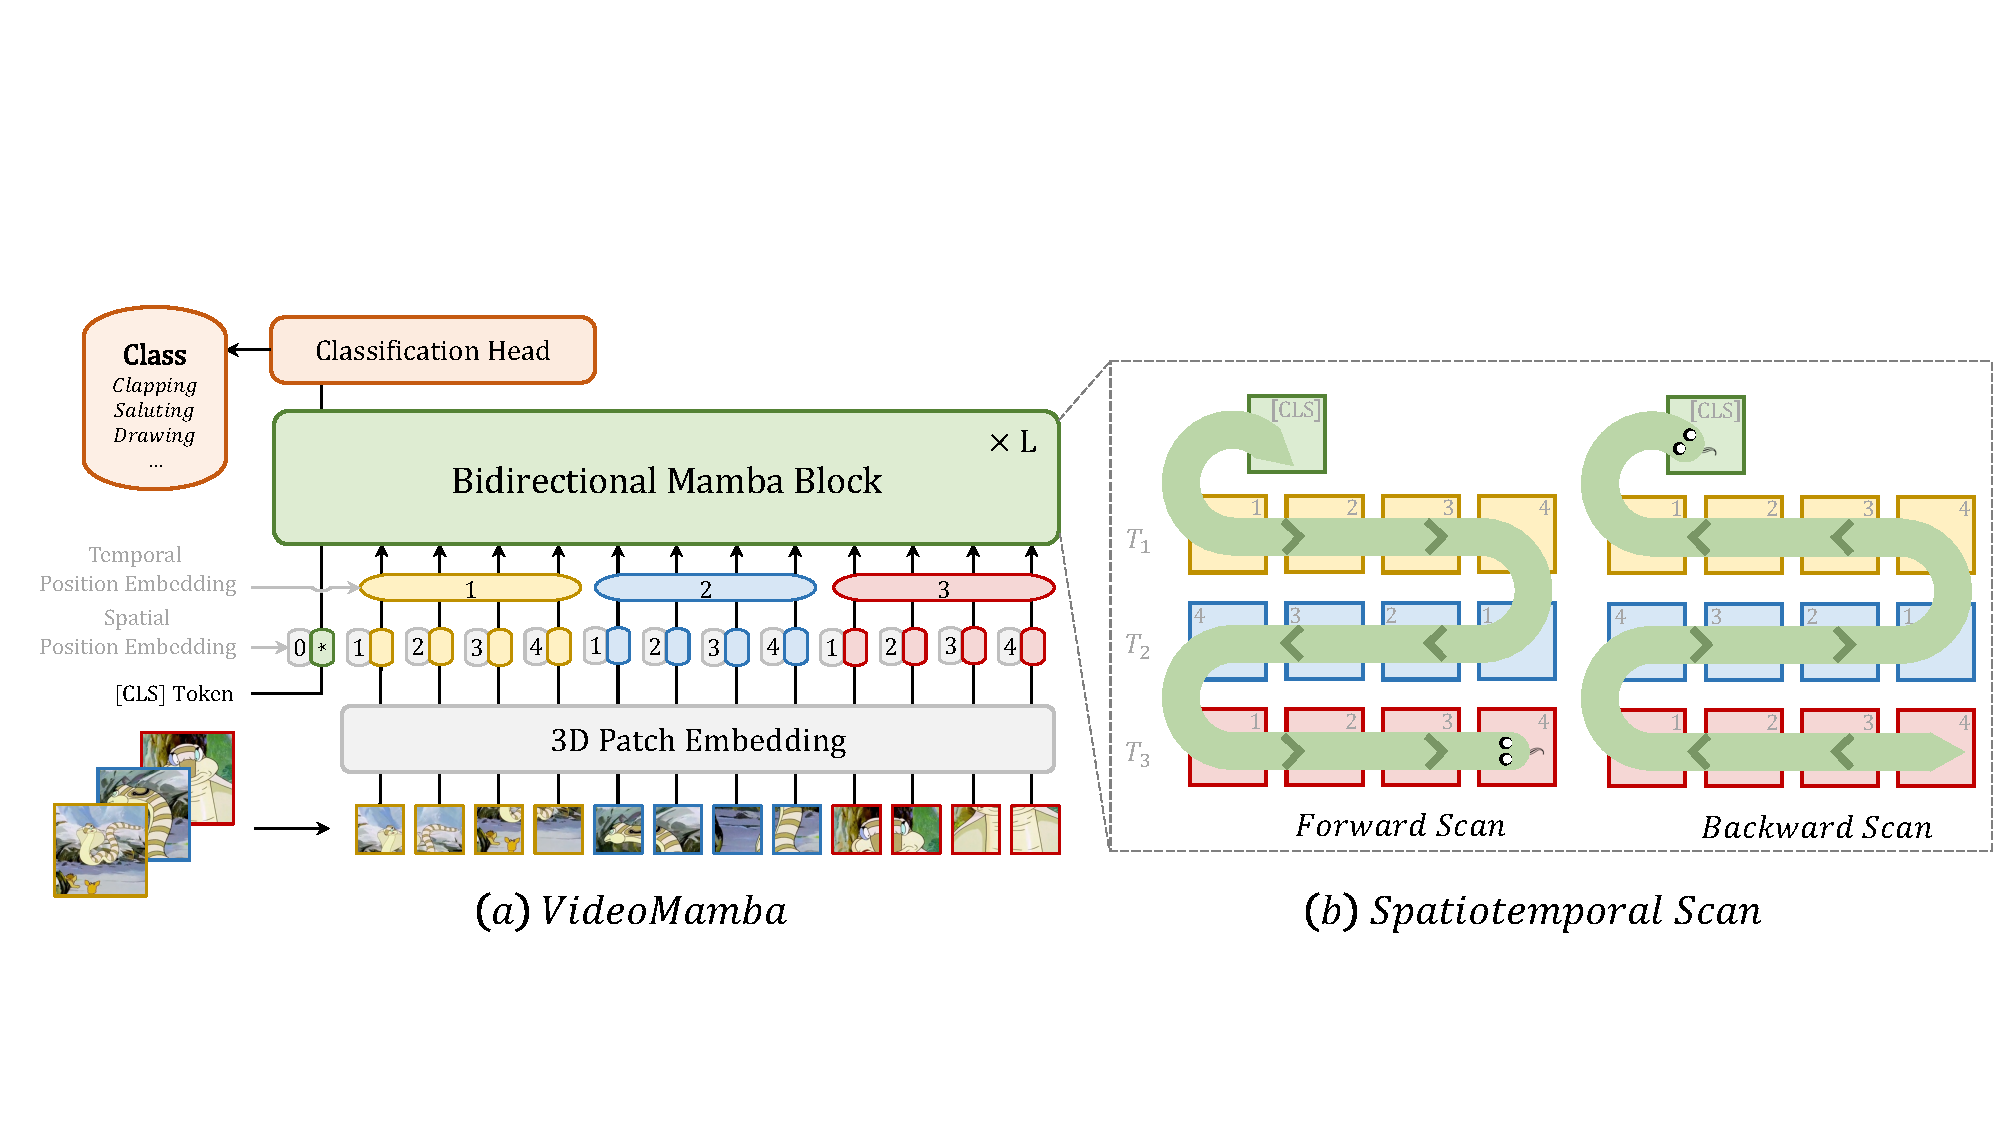
\includegraphics[width=1.0\textwidth]{figs/framework.pdf}
    \vspace{-0.7cm}
    \caption{
    \textbf{Framework of \ModelName.} 
    We strictly follow the architecture of vanilla ViT~\cite{vit}, and adapt the bidirectional mamba block\cite{vim} for 3D video sequences.
    % \textit{i.e.}, spatial-first scan.
    }
    \label{fig:framework}
    \vspace{-0.3cm}
\end{figure}


\subsection{\ModelName}


\noindent\textbf{Overview.}
Fig.~\ref{fig:framework} illustrates the overall framework of \ModelName.
Specifically,
we first use 3D convolution (\textit{i.e.}, 1$\times$16$\times$16) to project the input videos $\mathbf{X}^{v}\in \mathbb{R}^{3\times T\times H\times W}$ 
into $L$ non-overlapping spatiotemporal patches $\mathbf{X}^{p}\in \mathbb{R}^{L\times C}$,
where $L$$=$$t$$\times$$h$$\times$$w$ ($t$$=$$T$, $h$$=$$\frac{H}{16}$, and $w$$=$$\frac{W}{16}$).
The sequence of tokens input to the following \ModelName\  encoder is
\begin{align}
    \mathbf{X} ={}& \left[ \mathbf{X}_{cls}, \mathbf{X} \right] + \mathbf{p}_{s} + \mathbf{p}_{t},
\end{align}
where $\mathbf{X}_{cls}$ is a learnable classification token that is prepended to the start of the sequence.
Following previous works~\cite{vit,vivit,timesformer},
we added a learnable spatial position embedding $\mathbf{p}_{s} \in \mathbb{R}^{(hw+1) \times C}$ and the extra temporal one $\mathbf{p}_{t} \in \mathbb{R}^{t \times C}$ to retain the spatiotemporal position information,
since the SSM modeling is sensitive to token position.
The tokens $\mathbf{X}$ are then passed through by $L$ stacked B-Mamba blocks,
and the representation of ${\rm [CLS]}$ token at the final layer is processed by normalization and linear layer for classification.

\vspace{0.05cm}
\noindent\textbf{Spatiotemporal Scan.}
To apply the B-Mamba layer for spatiotemporal input,
we extend the original 2D scan into different bidirectional 3D scans in Fig. \ref{fig:scan}:
(a) \textit{Spatial-First}, organizing spatial tokens by location then stacking them frame by frame;
(b) \textit{Temporal-First}, arranging temporal tokens based on the frame then stacks along the spatial dimension;
(c) \textit{Spatiotemporal}, a hybrid of both \textit{Spatial-First} and \textit{Temporal-First}, with v1 conducting half of them and v2 conducting full of them ($2\times$ computation).
Moreover,
our experiments in Fig. \ref{tab:ablation_scan} demonstrate that the Spatial-First bidirectional scan is the most effective yet simple. 
Thanks to the linear complexity of Mamba,
our \ModelName\  is capable of handling long videos of high resolution efficiently. 


\begin{figure}[t]
    \centering
    \vspace{-0.3cm}
    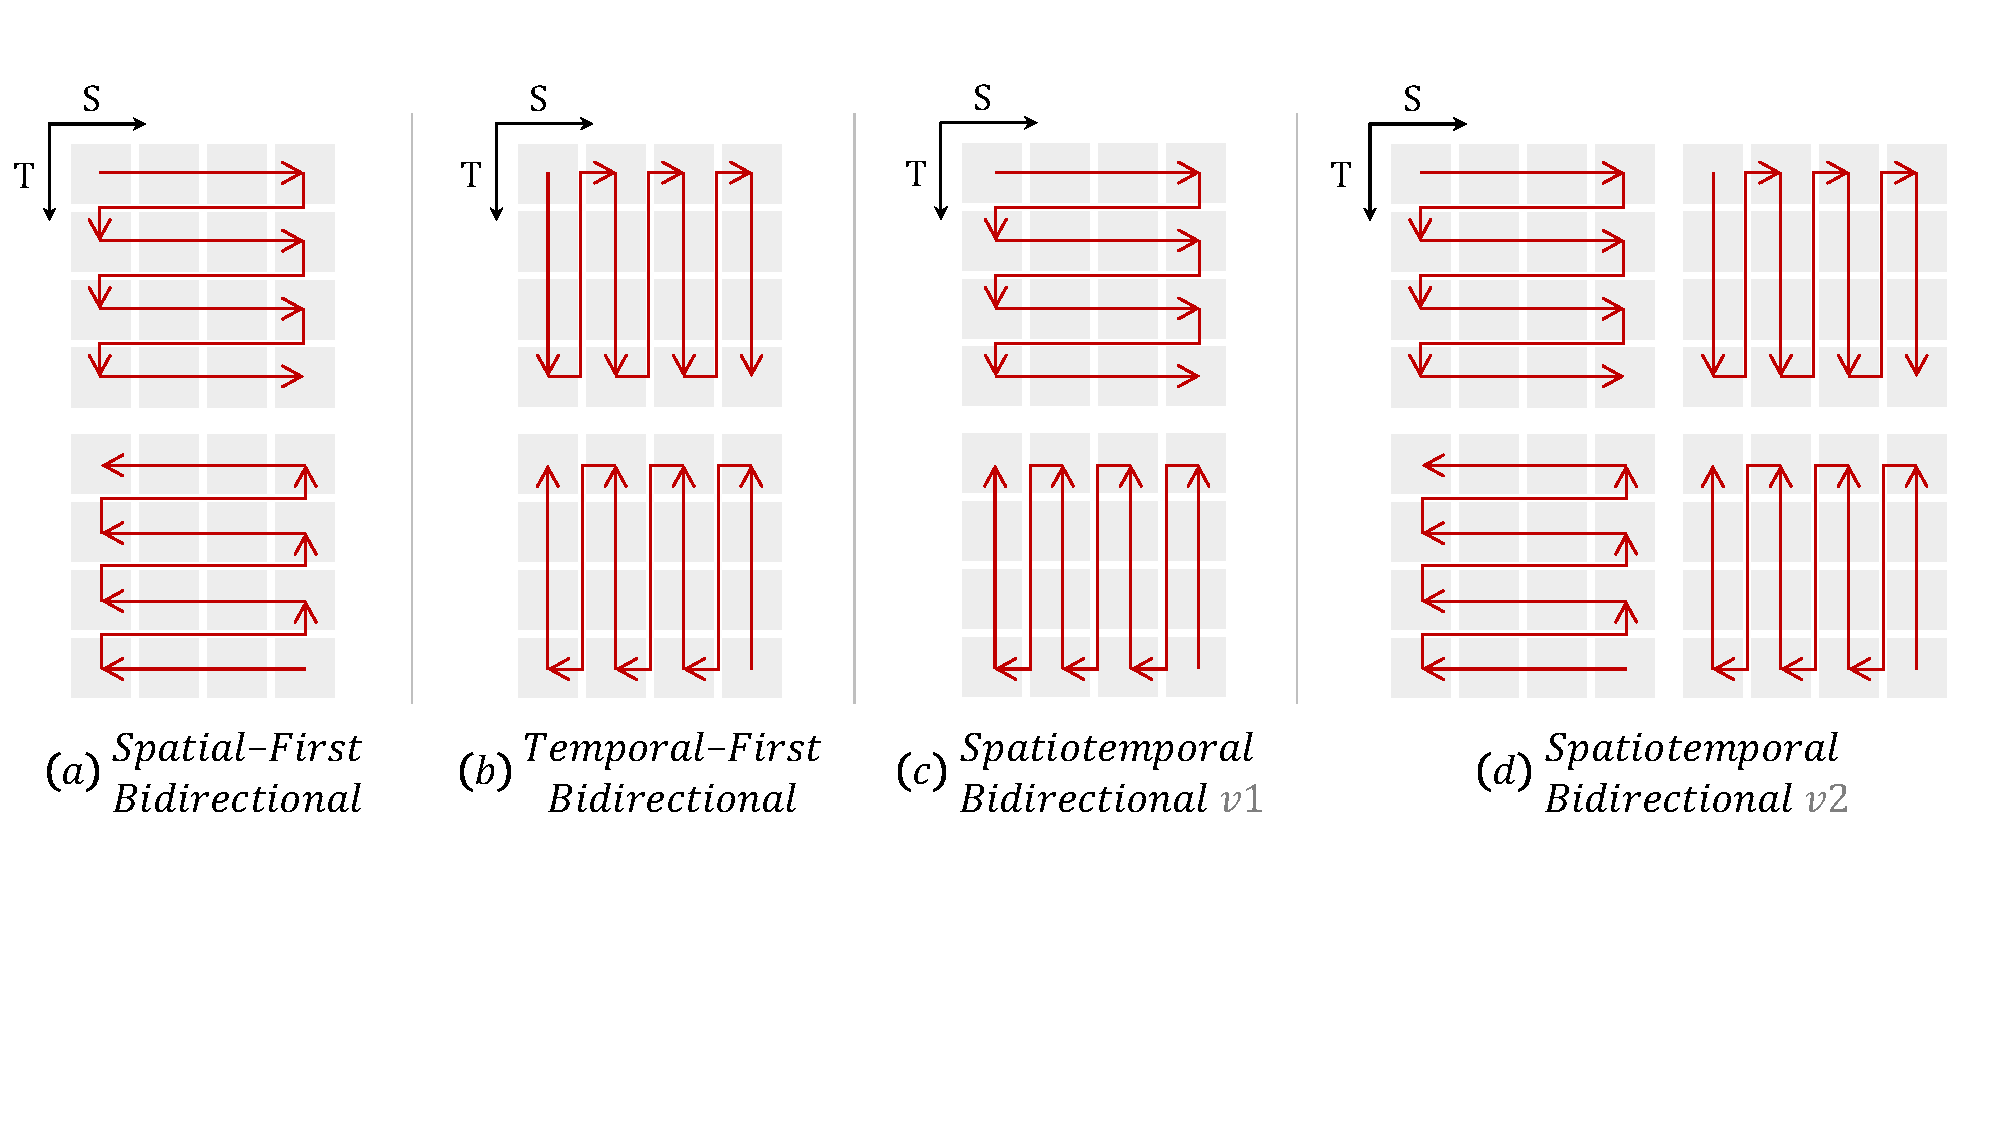
\includegraphics[width=1.0\textwidth]{figs/scan.pdf}
    \vspace{-0.7cm}
    \caption{
    \textbf{Different scan methods.}
    We omit the [CLS] token for simplification.
    }
    \label{fig:scan}
    \vspace{-0.3cm}
\end{figure}

\vspace{0.05cm}
\noindent\textbf{Comparison to Vim~\cite{vim} and VMamba~\cite{vmamba}.}
Our \ModelName\  builds upon Vim, 
yet streamlines its architecture by omitting features such as the middle [CLS] token and Rotary Position Embedding (RoPE~\cite{rope}), 
resulting in superior performance on ImageNet-1K with gains of \textbf{+0.8\%} and \textbf{+0.7\%} for Vim-Ti and Vim-S, respectively.
Unlike VMamba, 
which incorporates additional depthwise convolution, 
\ModelName\  strictly follows the ViT design without downsampling layers. 
To counter the overfitting issues observed in VMamba, 
we introduce an effective self-distillation technique outlined in Section~\ref{sec:arch},
demonstrate the isotropic \ModelName's great scalability for image and video tasks.


\vspace{0.05cm}
\noindent\textbf{Comparison to TimeSformer~\cite{timesformer} and ViViT~\cite{vivit}.}
Traditional attention-based models like TimeSformer and ViViT have addressed the self-attention mechanism's quadratic complexity by adopting divided spatiotemporal attention.
Despite being more efficient, 
it introduces additional parameters and underperforms compared to joint attention, 
particularly in scenarios involving masked pretraining~\cite{videomae,umt}. 
In contrast, 
\ModelName\  processes spatiotemporal tokens with linear complexity, 
outperforming TimeSformer on Kinetics-400 by \textbf{+2.6\%} and making significant strides on SthSthV2 with a \textbf{+5.9\%} improvement (see Table \ref{results_k400} and \ref{results_ssv2}). 
Furthermore, 
\ModelName\  achieves a \textbf{6$\times$} increase in processing speed and requires \textbf{40$\times$} less GPU memory for long videos, 
as detailed in Fig. \ref{fig:comparison_memory_speed}, 
demonstrating its efficiency and effectiveness in handling long-video tasks.


\subsection{Architecture}
\label{sec:arch}


\begin{wraptable}{r}{5cm}
  \vspace{-0.8cm}
  \centering
  \setlength\tabcolsep{4pt}
  \resizebox{0.43\textwidth}{!}{
  \begin{tabular}{lrrr}
    \Xhline{1.0pt}
    \small{\textbf{Model}} & \scriptsize{\textbf{\#Depth}} & \scriptsize{\textbf{\#Dim}} & \scriptsize{\textbf{\#Param.}} \\
    \Xhline{0.8pt}
    Tiny & 24 & 192 & 7M \\
    Small & 24 & 384 & 26M \\
    Middle & 32 & 576 & 74M \\
    \gray{Base} & \gray{24} & \gray{768} & \gray{98M}  \\
    \Xhline{1.0pt}
  \end{tabular}
  }
  \vspace{-0.2cm}
  \caption{\textbf{Different model sizes.} \gray{Base model is finally excluded} due to its suboptimization.} 
  \label{tab:model_size}
  \vspace{-0.6cm}
\end{wraptable}

For SSM in the B-Mamba layer,
we adopt the default hyperparameters as in Mamba~\cite{gu2023mamba}.
setting the state dimension and expansion ratio to 16 and 2, respectively.
Following ViT~\cite{vit},
we adjust the depth and embedding dimensions to create models of comparable sizes in Table \ref{tab:model_size}, 
including \ModelName-Ti, \ModelName-S and \ModelName-M. 
However, 
we observe that larger \ModelName\ tends to overfit during our experiments, 
leading to suboptimal performance as illustrated in Fig. \ref{tab:ablation_sd}\red{a}. 
This overfitting issue is not unique to our models but is also found in VMamba~\cite{vmamba}, 
where the optimal performance of VMamba-B was achieved at three-quarters of the total training epochs. 
To counteract the overfitting in larger Mamba models, 
we introduce an effective Self-Distillation strategy,
which uses a smaller and well-trained model as the ``teacher'' to guide the training of the larger ``student'' model. 
The results, depicted in Fig. \ref{tab:ablation_sd}\red{a}, show that this strategy leads to expected better convergence.

\subsection{Masked Modeling}

\begin{figure}[t]
    \centering
    \vspace{-0.3cm}
    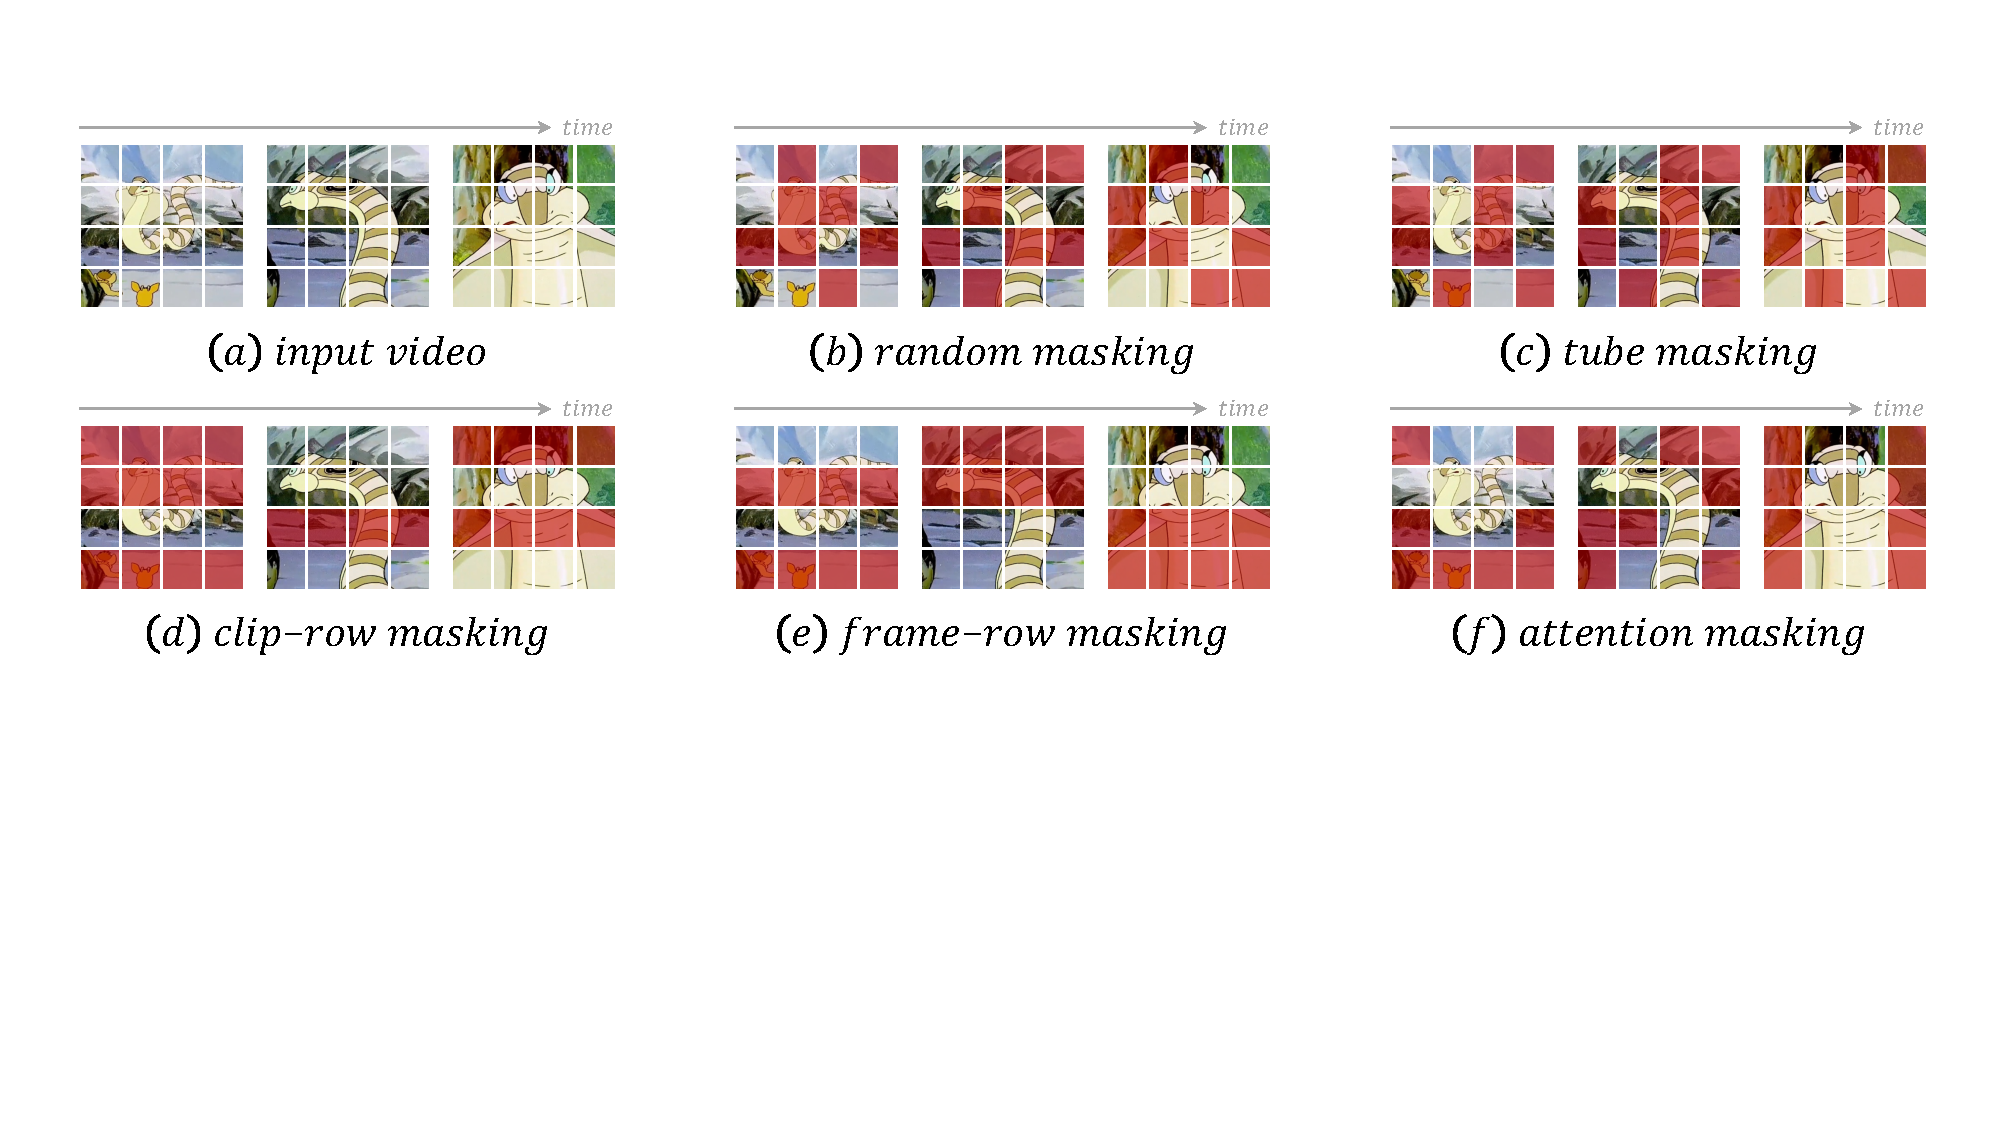
\includegraphics[width=1.0\textwidth]{figs/mask.pdf}
    \vspace{-0.6cm}
    \caption{
    \textbf{Different masking strategies.}
    Row masking, 
    tailored for \ModelName\ in light of the 1D convolution preceding SSM, 
    enhances performance with continuous tokens. 
    The difference between clip-row and frame-row masking is that the former masks the entire video clip, while the latter masks each frame individually.
    % Attention masking tends to preserve the adjacent region with meaningful information.   
    }
    \label{fig:mask}
    \vspace{-0.3cm}
\end{figure}

Recently, 
VideoMAE and ST-MAE~\cite{videomae,st_mae} have showcased the significant benefits of masked modeling in enhancing a model's capability for FINE-GRAINED temporal understanding. 
UMT~\cite{umt} takes this further by introducing an efficient masked alignment technique that yields robust results across single and multi-modal video tasks. 
To augment \ModelName's temporal sensitivity and verify its adaptability with text modalities, 
we adopt a masked alignment approach inspired by UMT. 
Firstly,
\ModelName\  is trained from scratch on video data alone, 
aligning unmasked tokens with those from CLIP-ViT. Subsequently, 
it is integrated with a text encoder and a cross-modal decoder (\textit{i.e.}, BERT~\cite{devlin2018bert}), 
for pretraining on both image-text and video-text datasets.

It's important to note the distinction from UMT, 
which employs multi-layer alignment between the student and teacher models. 
In contrast, 
due to \ModelName's unique architecture (SSM \textit{vs.} Transformer), 
we align only the final outputs. 
Regarding our masking strategy, 
we propose different row masking techniques, 
depicted in Fig.~\ref{fig:mask}, 
tailored to the B-Mamba block's preference for continuous tokens. 
Additionally, 
we explore attention masking to preserve meaningful adjacency among tokens, 
leveraging the inherent strengths of the 1D convolution within the B-Mamba block for improved performance.